\section{Conception}
    \subsection{Opérations importantes}
    \begin{itemize}
        \item a) Commandes/Ventes de plateau
        \item c) Approvisionnement et stockage
    \end{itemize}


\paragraph{Datamarts} 
    \begin{figure}[h]
        \centerline{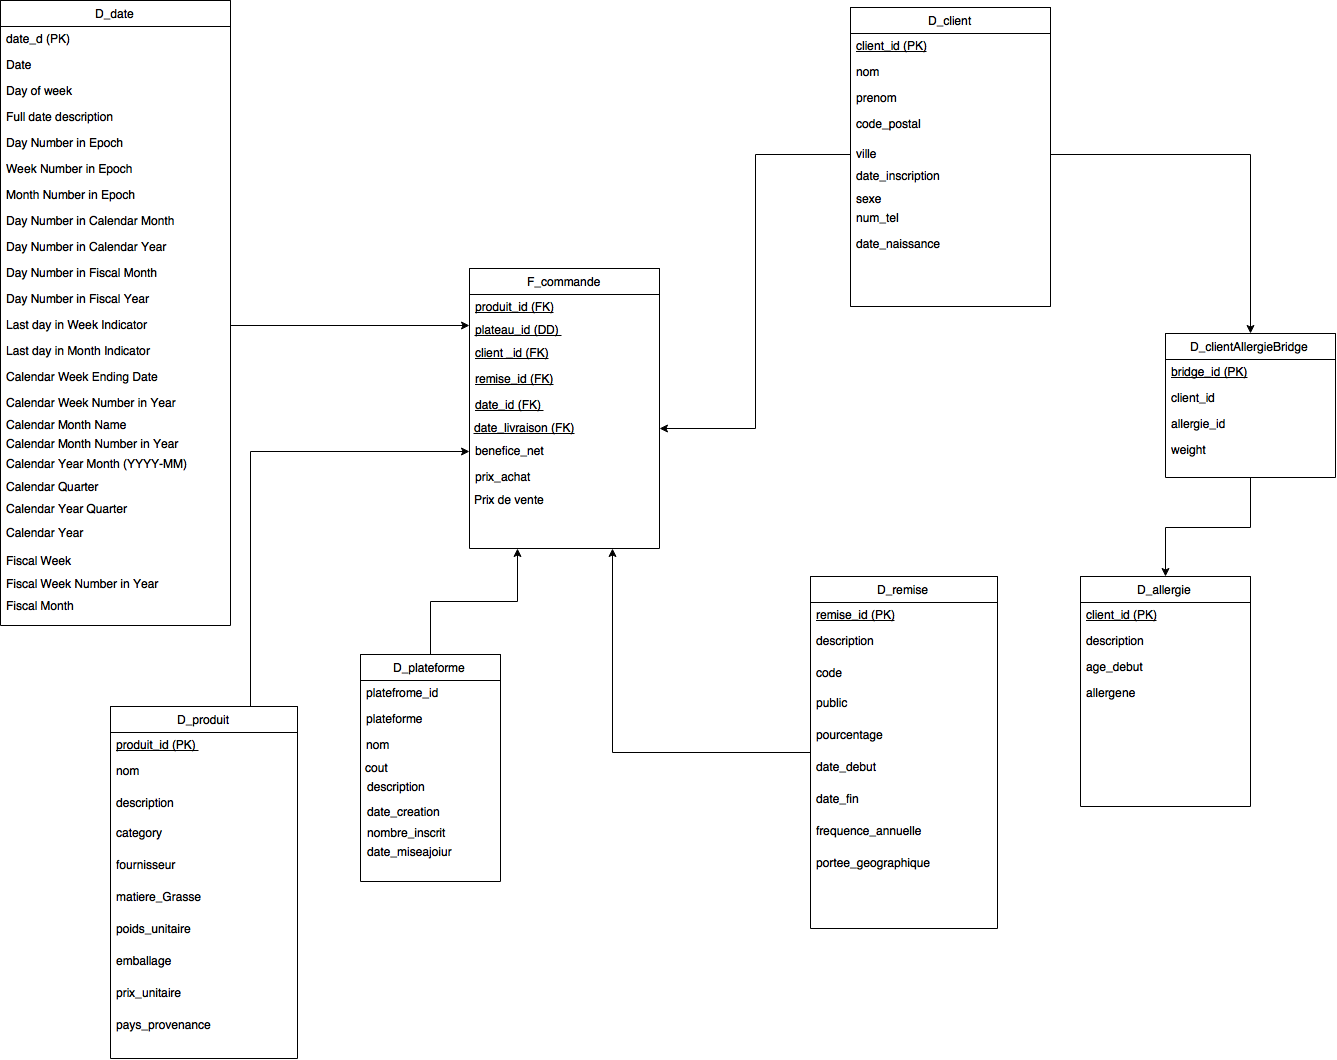
\includegraphics[scale=0.4]{EtoileDM1.png}}
        \caption{Premier Datamart}
        \label{fig:UML}
    \end{figure}
    
    \begin{figure}[h]
        \centerline{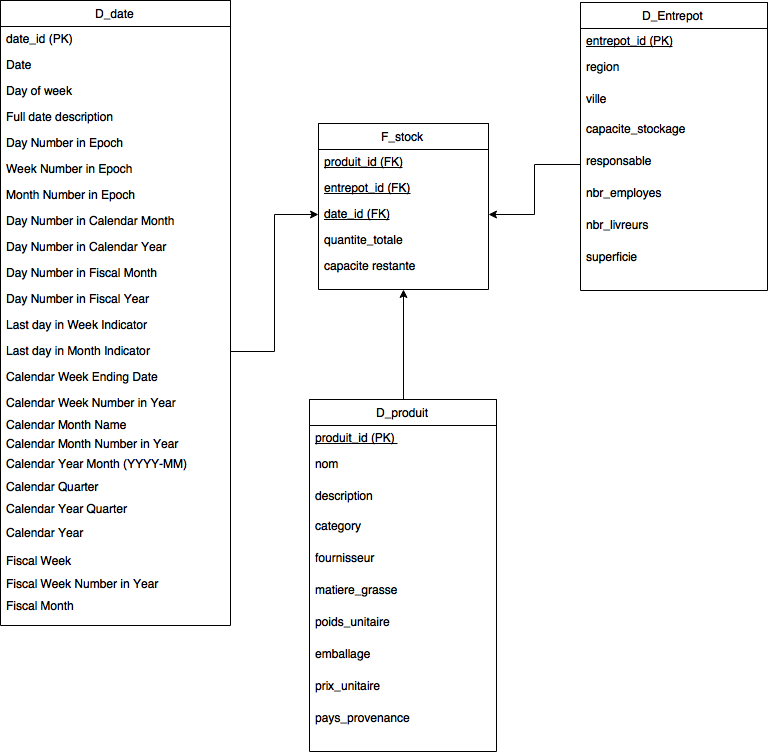
\includegraphics[scale=0.6]{EtoileDM2.png}}
        \caption{Deuxième Datamart}
        \label{fig:UML}
    \end{figure}

\paragraph{} Les mesures : Prix total et Bénéfice\_net sont toutes deux additives.

\paragraph{} 
Datamart opération c :
Il s’agit d’un snapshot périodique.
La mesure de capacité restante est semi-additive.

\subsection{Réponse aux requêtes} 
Le datamart peut être interrogé par les requêtes prévues.
